\documentclass[12pt]{article}
\usepackage[a4paper]{geometry}
\usepackage[myheadings]{fullpage}
\usepackage{amsmath,amssymb,amsthm, enumitem, hyperref, tabto} 
\usepackage{fancyhdr}
\usepackage{arxiv}
\usepackage{lastpage}
\usepackage{graphicx, wrapfig, subcaption, setspace}
\usepackage[font=small, labelfont=bf]{caption} \usepackage{blindtext}
 \usepackage{blindtext}
\usepackage{url, lipsum}
\usepackage{tgbonum}
\usepackage{amsmath,physics}
\usepackage{authblk}
\usepackage{hyperref}
 \hypersetup{ 
     colorlinks=true, 
     linkcolor=blue, 
     filecolor=blue, 
     citecolor =red,       
     urlcolor=cyan,
     pdftitle={Using Spatial Trees to optimize Food Costs for Lower Wage Families}
     } 
\usepackage[super,compress,sort,numbers]{natbib}
\usepackage{csquotes}
\usepackage{multicol}
%\setlength{\multicolsep}{6.0pt plus 2.0pt minus 1.5pt}% 50% of original values
\usepackage{xcolor}
\usepackage{algpseudocode}
\usepackage{algorithm}
\floatname{algorithm}{Algorithm}
\usepackage{times}
\usepackage{adjustbox}
\usepackage[T1]{fontenc}
\usepackage{makecell}
\usepackage{parskip}
\usepackage{erewhon}
\usepackage{geometry}
\usepackage{caption}
\usepackage{subcaption}
\usepackage{framed}
\setlength\FrameSep{0.5em}
\setlength\OuterFrameSep{\partopsep}
% \usepackage{draftwatermark}
\graphicspath{ {./images/} }
\usepackage{sectsty}

\sectionfont{\fontsize{15}{20}\selectfont}
\usepackage{tikz}
\def\checkmark{\tikz\fill[scale=0.4](0,.35) -- (.25,0) -- (1,.7) -- (.25,.15) -- cycle;} 
\usepackage[sorting=none]{biblatex}
\addbibresource{references.bib}

\newcommand{\HRule}[1]{\rule{\linewidth}{#1}}
\onehalfspacing
\setcounter{tocdepth}{5}
\setcounter{secnumdepth}{5}

\renewcommand{\headrulewidth}{0pt}
\renewcommand{\footrulewidth}{0pt}

\begin{document}


\pagestyle{fancy}
\fancyhf{}
\fancyhead[L]{\footnotesize \textbf{CS5132} PA2 - \emph{Using Spatial Trees to optimize Food Costs for Lower Wage Families} }

\fancyfoot[R]{Page \thepage\ of \pageref{LastPage}}


{\selectfont
\title{
	\huge \textbf{Using Spatial Trees to optimize Food Costs for Lower Wage Families}
}

\date{}

\author[1]{Kannan Vishal}
\author[1]{Prannaya Gupta}
\author[1]{Quek Yu Pin}
\author[1]{Vikram Ramanathan}
\affil[1]{NUS High School of Math and Science}

\maketitle

\vspace{-2cm}

\tableofcontents

\thispagestyle{empty}
\newpage

\section{Background}

    Food expenses make up a large proportion of the monthly expenditures of lower income families. However, as they decide where to buy their groceries or what to get for dinner, they will tend to go to the supermarket that is close to their homes. However, sometimes they may be better off walking a little further to shop at an NTUC, rather than at the Cold Storage branch which marks up its products. When a family is visiting a new neighbourhood, they may not even be sure where they can get takeout for an affordable price. Thus, we seek to present the options in a concise interface that optimizes for price and distance, so that users can make more informed decisions on their food expenditures. 
    
    % Explain the use of spatial trees
    
   
\section{User Documentation}
You are to provide a brief user documentation with \textbf{screenshots} on how to use the
program and its functionalities.

\section{Analysis and Explanation of Implemented Tree Methods}

Provide a brief explanation, in your own words, and rigorous mathematical worst-case
analysis derivation and time complexity of the key methods of your tree structure
(retrieval, insertion, deletion, balance (if any))




\subsection{Spatial Quad-Trees}
\begin{figure}[H]
    \centering
    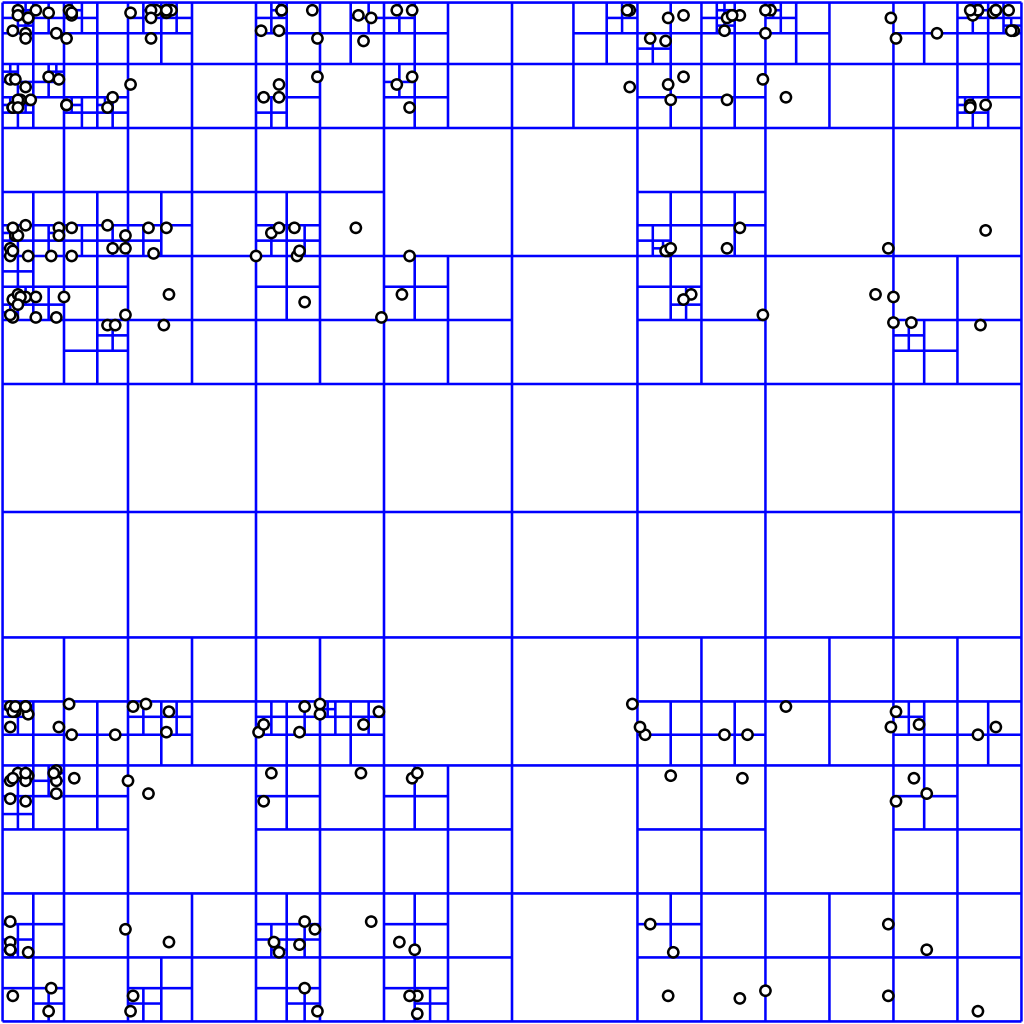
\includegraphics[width=\textwidth]{../img/quadtree.png}
    \caption{Quad-Tree visualization}
    \label{fig:my_label}
\end{figure}
Quad-Trees are commonly used in analysing the distribution of a collection in 2D space, as the size and precision of the data structure scales with the distribution of the spatial data we are working with. As we map out store branches over Singapore, we may find that the locations are not evenly distributed. If we try to split up the map of Singapore into a grid, and check if each grid is occupied by a store, then we may have a lot of overlap of stores in shopping districts, and wasted space in more residential areas. 

Quad-Trees address this by also splitting up the map into four quadrants and recursively making quadrants within those quadrants, but lazily. That is, a quadrant is subdivided only during when there is a child node to be inserted into the quadrant. The depth of the tree is thus proportional to the density of points, which results in many speedups.

\subsubsection{Algorithm}

In terms of implementation, Quad-Trees are essentially self-balancing binary search trees where the internal nodes have degree four instead of two. Thus we will focus on tree rotation, which is 

\subsection{Spatial R-Trees}

\begin{figure}[H]
    \centering
    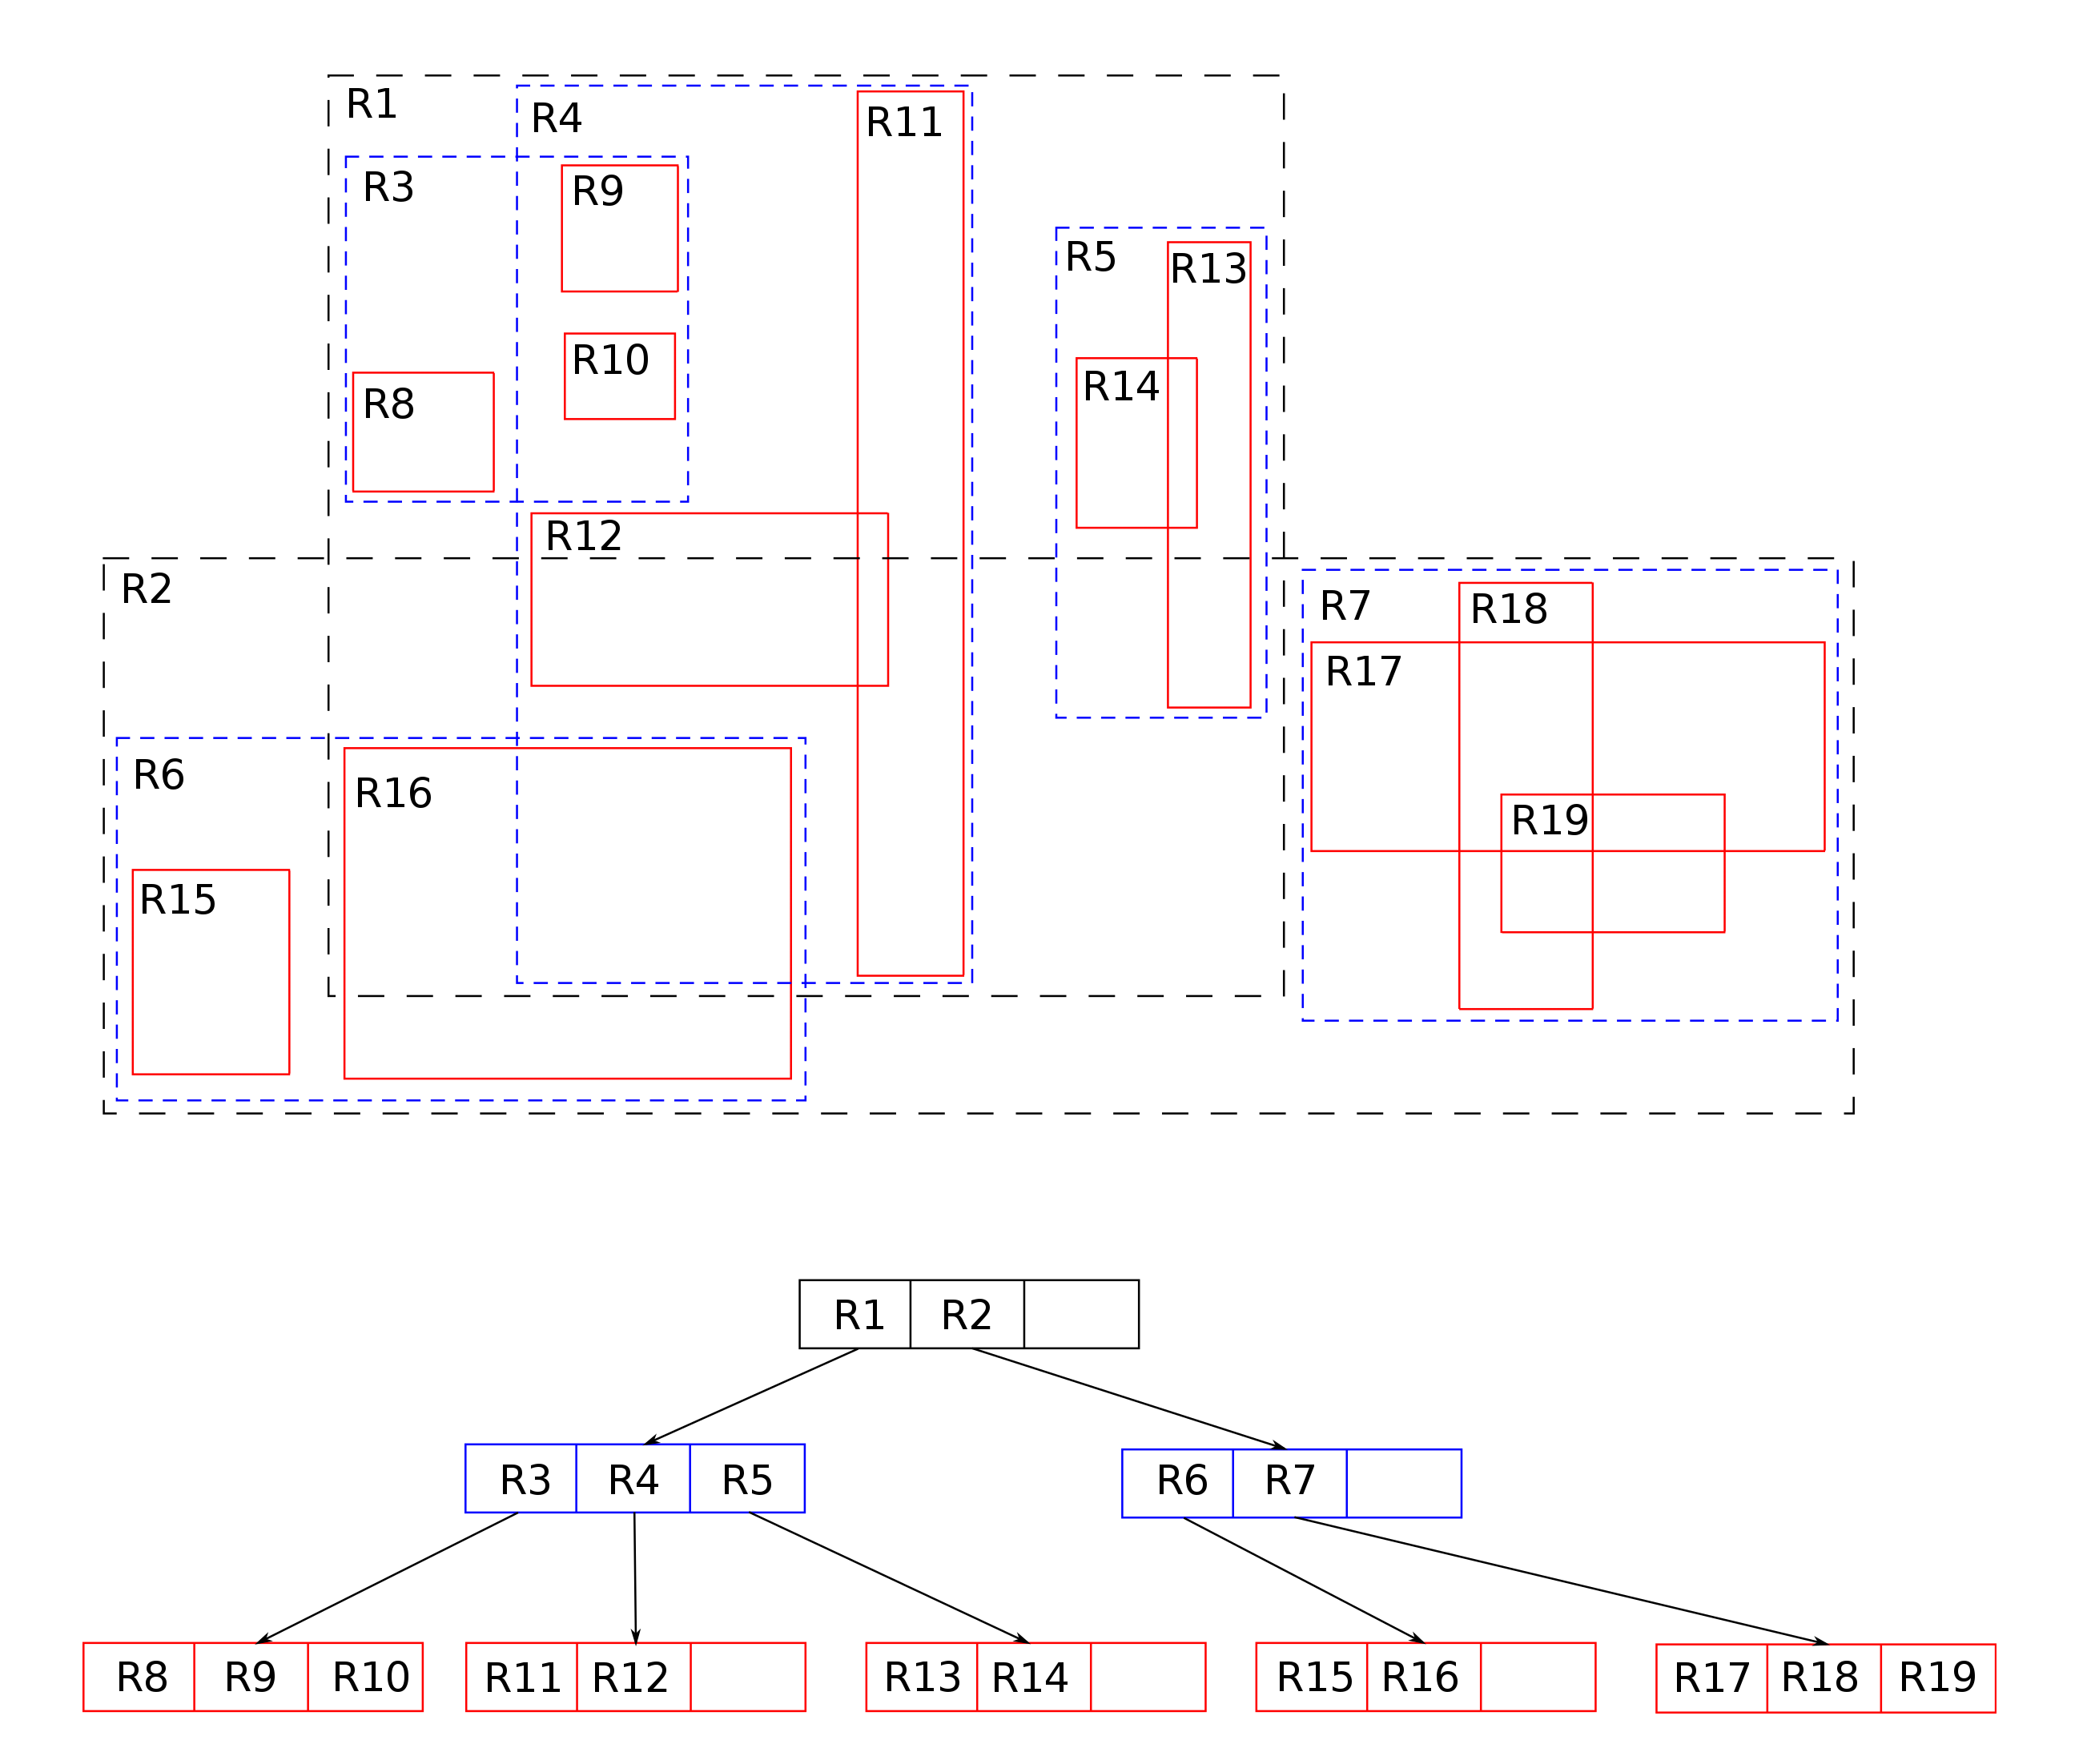
\includegraphics[width=\textwidth]{../img/RTree.png}
    \caption{R-Tree visualization}
    \label{fig:my_label}
\end{figure}

Another approach to storing points in space, especially for our purposes of nearest neighbour queries, is to group points together, according to their closeness, and then recursively group those groups together. 

\subsubsection{Algorithm}



\subsection{R-Trees vs. Quad-Trees}

% Hypothesis
% Why we think one would work better

\section{Testing Strategy}
You are to provide at least \textbf{3 test cases} you used to test the correctness and
robustness of your program. Log down the sample input and output for each test case.
Briefly explain why each test case was chosen.


\section{Results}

% Which data structure did better

\newpage
\section{GitHub Information}
You can find our repository at \url{https://github.com/ThePyProgrammer/SnackNow}.

\subsection{User Directory}
\begin{center}
    \begin{tabular}{|c|c|}
        \hline
        GitHub Username & Real Name \\
        \hline
        \href{https://github.com/delargement}{\texttt{delargement}} & Kannan Vishal \\
        \href{https://github.com/ThePyProgrammer}{\texttt{ThePyProgrammer}} & Prannaya Gupta \\
        \href{https://github.com/h1810126}{\texttt{h1810126}} & Quek Yu Pin \\
        \href{https://github.com/VikramRamanathan}{\texttt{VikramRamanathan}} & Vikram Ramanathan \\
        \hline
    \end{tabular}
\end{center}


\subsection{Repo Report}

\section{Reflection}

\subsection{Vishal}

By helping out a here and there in each component of the project, and reviewing our project while writing the report, I have gained a better understanding of the software development lifecycle, from the brainstorming stage, UI prototyping stage, data collection and documentation. By abstracting each component of the project, such as the model (RTree and Quadtree implementation) and GUI, and distributing the workload, we were able to be more productive, and it was enjoyable to see each of the pieces to connect together to give a minimum viable product.

\subsection{Prannaya}

\subsection{Yu Pin}

\subsection{Vikram}

\section{Work Distribution Matrix}

\begin{center}
\begin{tabular}{|c|c|c|c|c|}
    \hline
    & Vishal & Prannaya & Yu Pin & Vikram \\ [0.5ex] 
    \hline\hline
    Ideation & &  &  & \checkmark \\
    R-Tree Implementation &  & \checkmark &  & \checkmark \\
    Quad-Tree Implementation &  &  &  & \checkmark \\
    Data Collection &  &  & \checkmark &  \\
    User Interface  & \checkmark & \checkmark &  &  \\
    Report  & \checkmark &  &  &  \\
    \hline
\end{tabular}
\end{center}


\newpage


\section{References}

\printbibliography[
heading=none
]
}

\end{document}